\section{Introduction}

\begin{figure}[t]  
    \centering  
    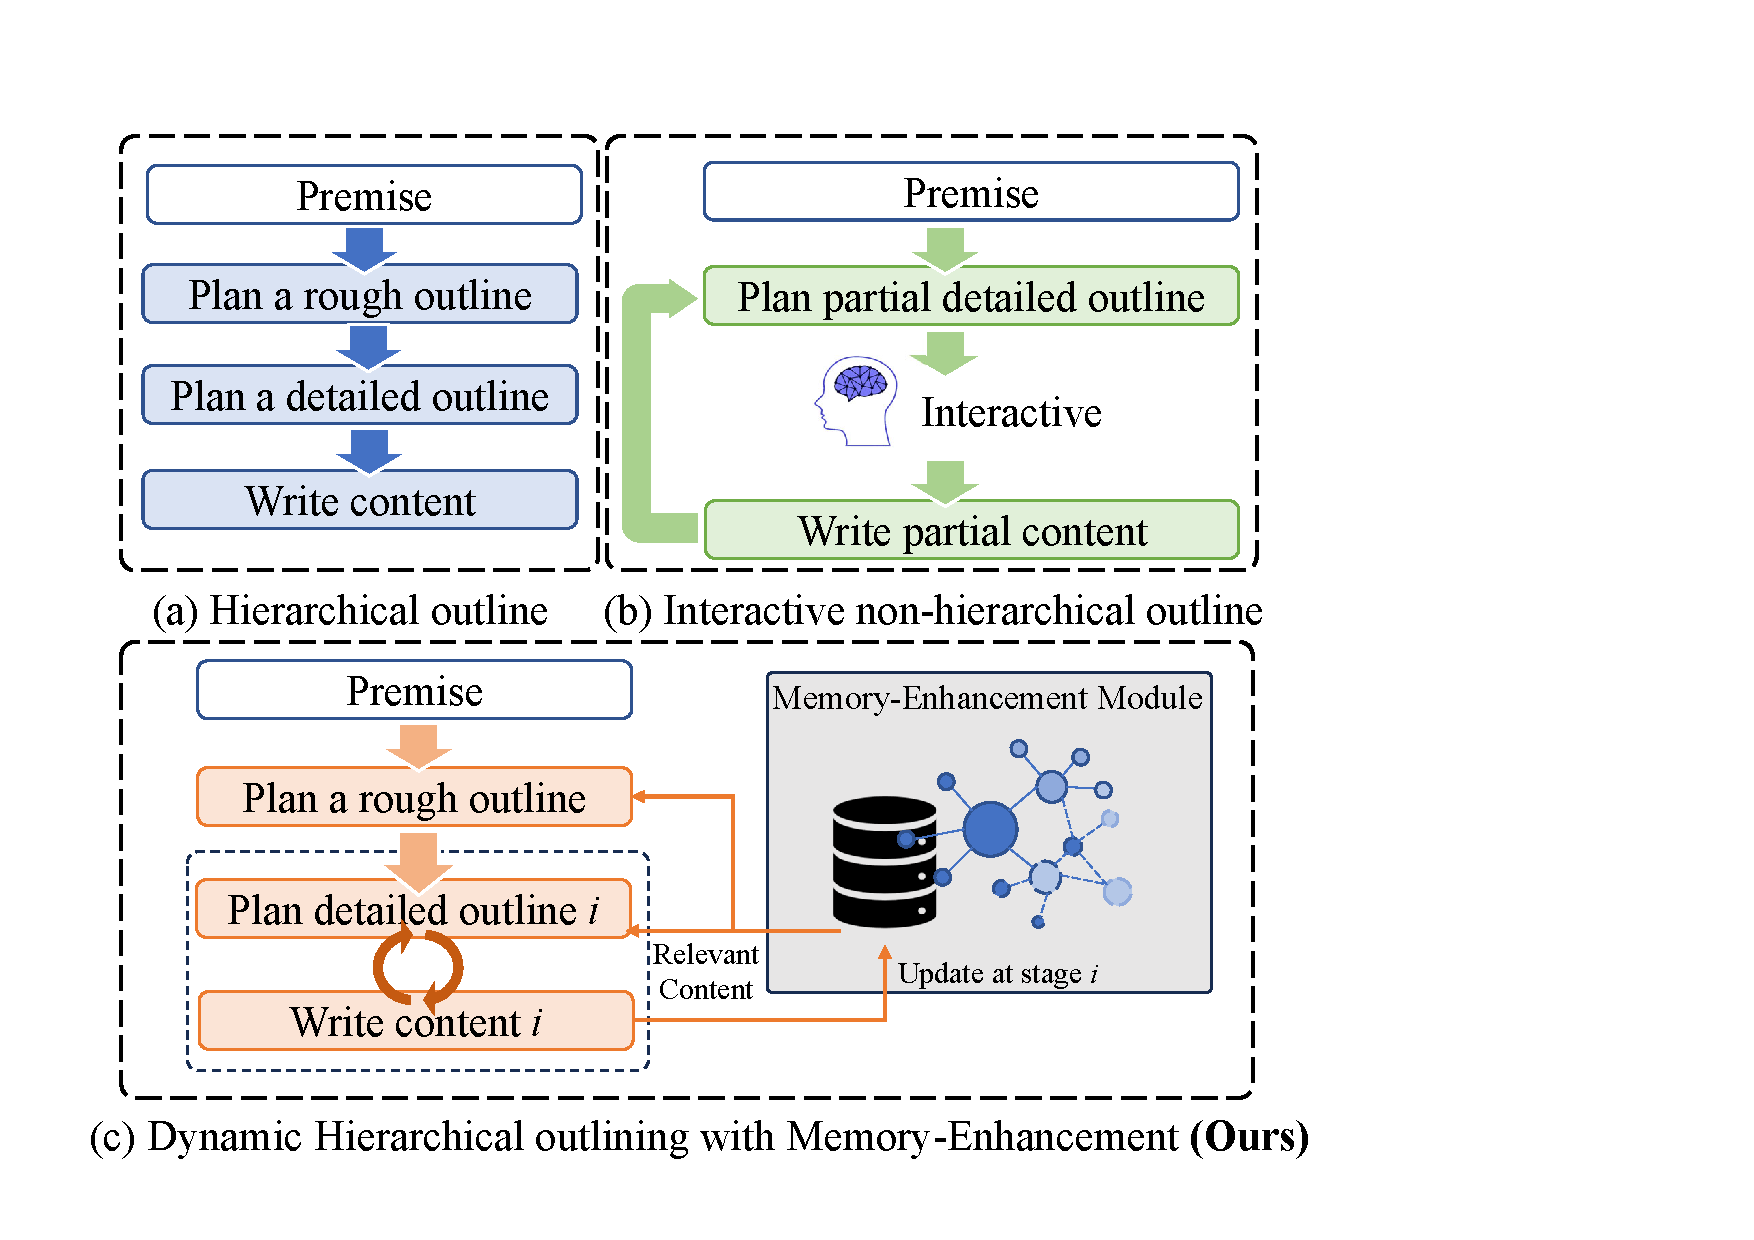
\includegraphics[scale=0.36]{images/Methods_compare.pdf}  
    \caption{Illustration and comparison of three strategies of long-form story generation. (a) applying a fixed hierarchical outline to guide the story generation, which is challenging to adapt to the uncertainty in story creation. (b) adapting to the uncertainty through interaction with humans, which allows for flexibility but lacks a high-level storyline to guide story development. Our method shown in (c) aims to enhance story coherence from both plot and expression and enjoys the advantages of the former two strategies to improve the coherence of the plot and reduce contextual conflicts.}  
    \label{method_compare}
    \vspace{-0.5cm}    
\end{figure} 

\hjw{Among natural language processing (NLP) tasks, the automatic generation of a long-form story is a representative task that requires creativity and long-term planning skills. By learning from human-written stories, an automated storyteller mimics humans and becomes competent in producing stories useful for various application scenarios, such as novel writing and interactive storytelling~\cite{riedl2010narrative}. Large Language Models (LLMs) are rapidly developing, generating a long-form story that further increases dramatically in length, complexity, and fluency~\cite{Re3}.} 


Unfortunately, it is difficult for the LLMs to generate a long-form story maintaining contextual consistency in semantic and coherent plot development for the following reasons. 1) \textit{Memory limitations}: The black-box self-attention mechanism forms the core of LLMs for contextual connections and still suffers from the long-range dependency issue~\cite{vaswani2017attention}, making it hard for them to precisely and unambiguously recall and thereby leading to contextual incoherence. 2) \textit{Planning difficulties}: LLMs cannot effectively apply knowledge of coherent plot planning partly because their training involves learning from vast datasets that include a variety of texts, but they do not inherently understand or apply the principles of storytelling and thus hinders the generation of engaging stories with complete and fluent plots~\cite{xie-etal-2023-next}


\hjw{Existing long-form story generation methods often leverage higher-level attributes such as plots or commonsense knowledge~\cite{xie-etal-2023-next}, primarily aiming to enhance story development fluency, and can be divided into two kinds based on whether humans are involved. The first category emulates the human writing process by adopting a plan-and-write framework~\cite{Re3} in generating the long-form story (see Fig. \ref{method_compare}(a)). This approach separates the generation process into the planning and writing stages, utilizing detailed and plot-fluent outlines to guide the writing phase. While these methods can extend the length of the story and improve plot development fluency, the inflexibility of a fixed outline can impede its adaptability to uncertainty in the writing stage, often leading to plot incoherence, such as contextual repetition or conflicts.}Other works ~\cite{RecurrentGPT,brahman2020cue} explore generating content progressively without outlining based on human interaction and relevant preceding content \hjw{(see Fig. \ref{method_compare} (b))}. They can address the influence of local plot development caused by uncertainty in generation. However, the generated story lacks a macro-level of rational planning, affecting the plot completeness.



\hjw{To address the above limitations, we propose \textbf{D}ynamic Hierarchical \textbf{O}utlining with \textbf{M}emory-\textbf{E}nhancement long-form story generation method, called \textbf{DOME}, to generate the long-form story with coherent content and plot (see Fig. \ref{method_compare}(c)). \wqyr{\textbf{DOME} is based on the collaboration of a Dynamic Hierarchical Outline (DHO) mechanism and a Memory-Enhancement Module (MEM) to generate long-form story.}
Specifically, DHO mechanism to guide long-form story generation based on the plan-write writing framework~\cite{Re3} and the novel-writing theory \cite{TheoryFive}. The DHO mechanism requires the generation of a rough outline conforming to the novel writing theory to ensure plot completeness, and the dynamic planning of a detailed outline based on the rough outline during the writing process so that it can adapt to the uncertainty of the generation and improve the plot fluency. The MEM stores and accesses generated stories through temporal knowledge graphs and provides contextual content for outline planning and story writing to reduce content conflicts in long story texts. \wqyr{To automatically evaluate the contextual consistency, we propose a conflict detection matrix (named Temporal Conflict Analyzer) based on the information representation rules of the temporal knowledge graph and LLM.}}




\hjw{Our main contributions are as follows:}

\begin{itemize}
\vspace{-6pt}
\item 

\hjw{\textbf{A new paradigm for long-form story generation.} 
\wqyr{Since we find that existing methods for long-form story generation either cause plot incoherence due to fixed outlines or lack of fluency and readability due to poor macro-level planning, we propose a dynamic hierarchical outline (DHO) mechanism to fuse the planning and writing stages, making it adaptable to the generation uncertainty and improving plot coherence. Experiments show that DHO improves 6.87\% on ${Ent}$-2 metric.}}

\vspace{-6pt}
\item
\hjw{\textbf{A new approach to contextual conflict resolution.} We propose a Memory-enhancement module (MEM) based on the temporal knowledge graph to store and access the generated story. \wqyr{Applying LLM to perform semantic filtering on KG retrieval results keeps the conciseness of historical information and thus improves the contextual consistency of generated stories. 
}
Experiments show that MEM reduces conflicts by 87.61\%.}

\vspace{-6pt}
\item 
\textbf{A new evaluation for conflict detection.} To evaluate the degree of contextual consistency automatically, we propose a potential conflict detection method based on the information representation rules of the temporal knowledge graph and apply LLM to further determine whether a conflict exists. 
\wqyr{Experiments show that the judgment results of this method are consistent with human preferences.}

\end{itemize}

\begin{figure*}[t]

	\centering
	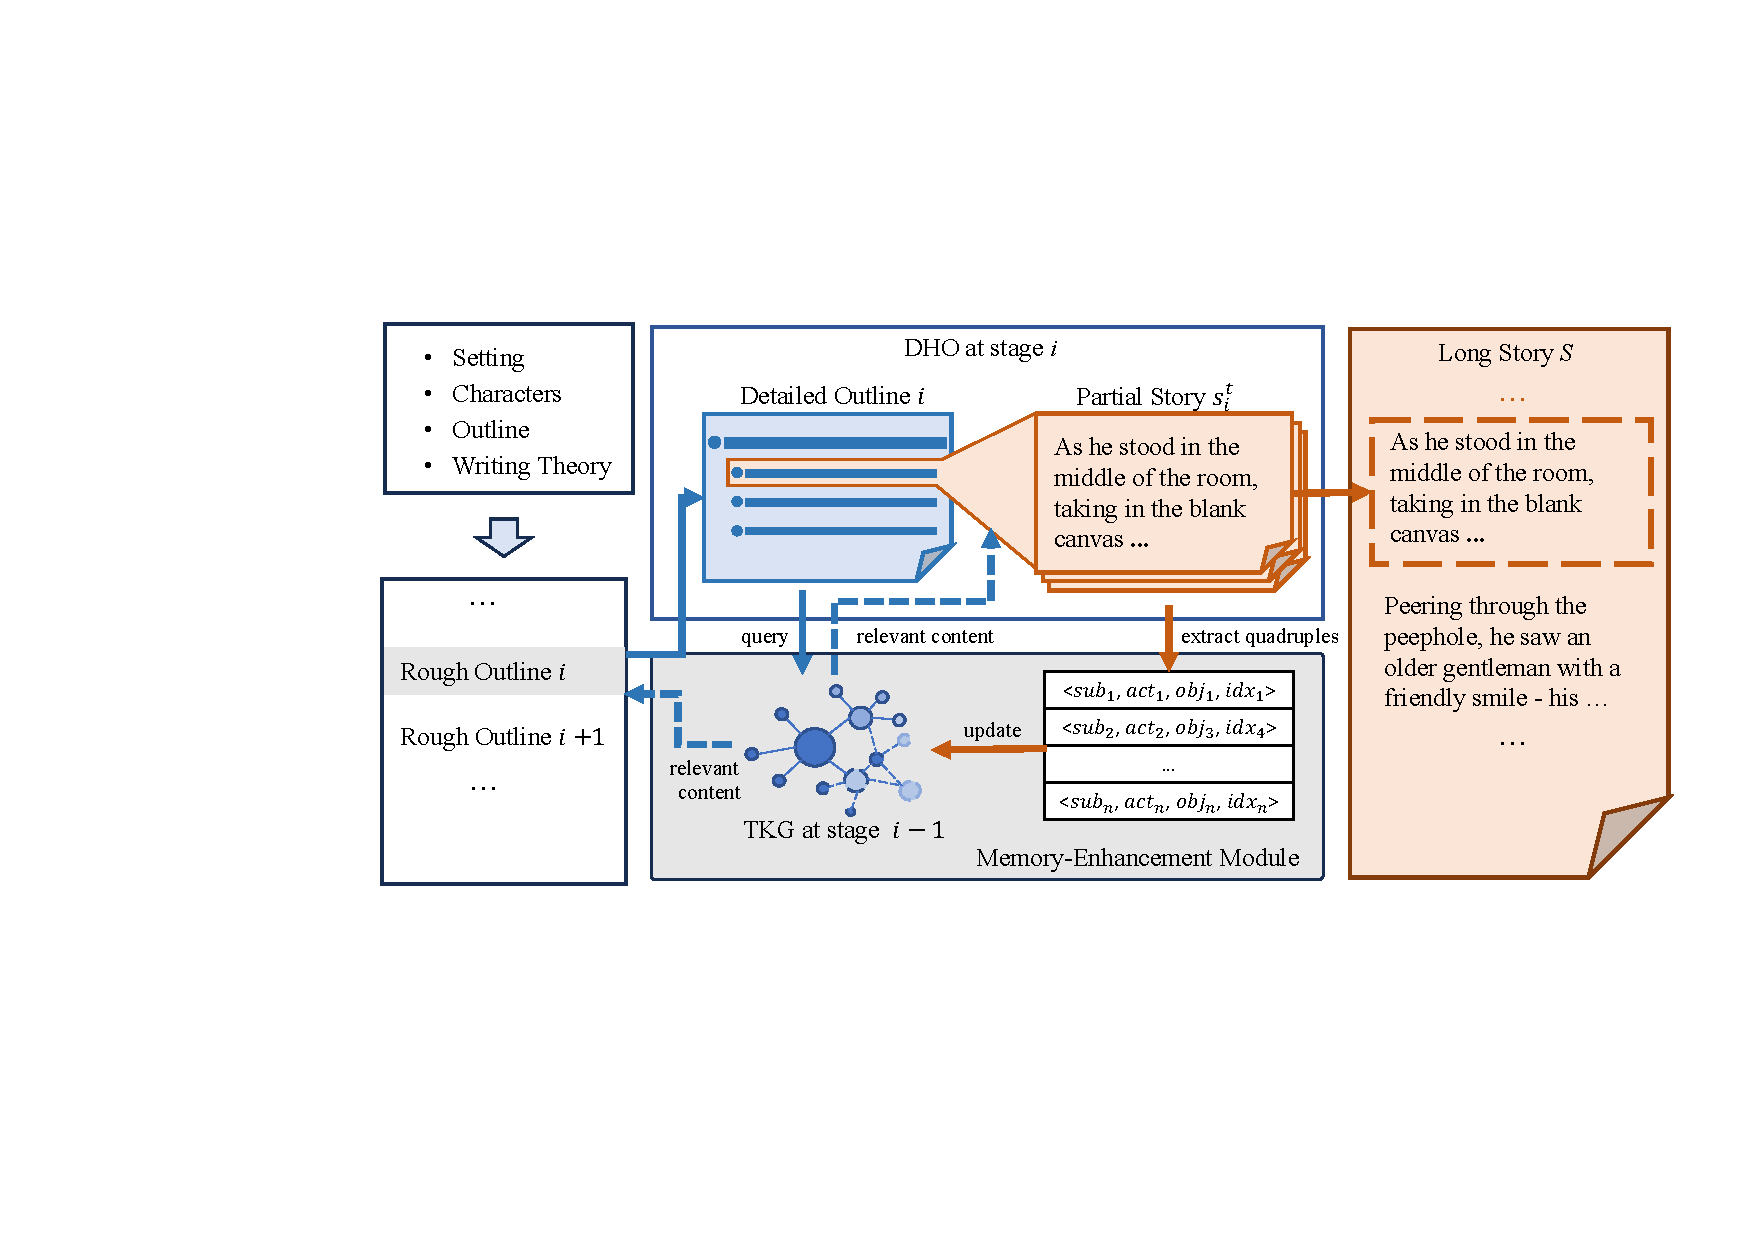
\includegraphics[width=0.96\textwidth]{images/our_method3.pdf}
	\caption{General diagram of proposed \methodname. The story generation process is divided into several stages based on the amount of rough outline.  At stage $i$, we expand rough outline $i$ into several detailed outlines based on the relevant content provided by MEM, and these outlines generate partial story sequentially based on their relevant content querying from MEM. Every generated partial story is stored in a temporal Knowledge graph for the following query.}
	\label{fig:our_method}
 \vspace{-6pt}
\end{figure*}

